\documentclass{article}
\usepackage[english,greek, main=greek]{babel}
\usepackage[utf8]{inputenc}

\usepackage{amsmath}
\usepackage{chngcntr}
\counterwithin{equation}{section}

\usepackage{graphicx}
\usepackage{subcaption}
\usepackage{placeins}

\newcommand{\eng}[1]{\foreignlanguage{english}{#1}}
\newcommand{\Alpha}{\mathrm{A}}

\useshorthands{;}
\defineshorthand{;}{?}

\title{Όραση Υπολογιστών\\
        \large Εργαστήριο 1}
\author{Αναστάσιος Στέφανος Αναγνώστου\\
    \texttt{03119051}
        \and
        Σπυρίδων Παπαδόπουλος\\
    \texttt{03119058}}

\date{7 Απριλίου 2023}

\begin{document}
\maketitle

\newpage
\tableofcontents
\newpage

\section{Μέρος 1ο}

\subsection{Δημιουργία Εικόνων Εισόδου}

Οι εικόνες εισόδου δημιουργούνται διαβάζοντας την δεδομένη εικόνα ''\eng{edgetest\_23.png}`` και προσθέτοντας θόρυβο σε αυτήν. Προστίθεται αντιστοίχως θόρυβος με \eng{PSNR} 20\eng{dB} και θόρυβος με \eng{PSNR} 10\eng{dB}. Αξιοσημειώτο είναι, ότι ο πρώτος θόρυβος είναι στην πραγματικότητα λιγότερος από τον δεύτερον. Το \eng{PSNR} ορίζεται ως εξής:

\begin{equation}
    \begin{gathered}
        PSNR = 20\log_{10} \left(\frac{I_{max}-I_{min}}{\sigma_n} \right)(dB),\\
        I_{max} = \underset{x,y} {\max} I(x,y), I_{min} = \underset{x,y} {\min} I(x,y)
    \end{gathered}
\end{equation}

Φαίνεται ότι από τον ορισμό μπορεί να ληφθεί η μεταβλητότητα του θορύβου, βάσει της οποίας τελικά αυτός ορίζεται. Από την έκφραση της μεταβλητότας, μάλιστα, φαίνεται ότι, όσο μεγαλύτερο το \eng{PSNR} σε \eng{dB} τόσο μικρότερη είναι τελικά η μεταβλητότητα του θορύβου, πράγμα που επαληθεύει τα προαναφερθέντα.

\begin{equation}
    \sigma_n = \frac{\left(I_{max}-I_{min}\right)}{10^{\frac{PSNR}{20}}}
\end{equation}

\subsection{Υλοποίηση Αλγορίθμων Ανίχνευσης Ακμών}

Η συνάρτηση που θα αναπτυχθεί εφαρμόζει είτε γραμμική είτε μη γραμμική μέθοδο ανίχνευσης ακμών.

\subsubsection{Γραμμική Μέθοδος}

Η μεν γραμμική μέθοδος επιχειρεί την προσέγγιση της λαπλασιανής της εξομαλυμένης εικόνας χρήσει γραμμικών φίλτρων. Συγκεκριμένα, σύμφωνα με την γραμμική μέθοδο:

\begin{equation}
    L = \nabla^2 \left(G_{\sigma} * I\right) = \left( \nabla^2 G_{\sigma} \right) * I
\end{equation}

\subsubsection{Μη Γραμμική Μέθοδος}

Η δε μη γραμμική μέθοδος επιχειρεί την προσέγγιση της λαπλασιανής της εξομαλυμένης εικόνας χρήσει μορφολογικών τελεστών. Συγκεκριμένα, σύμφωνα με την μη γραμμική μέθοδο:

\begin{equation}
    \begin{gathered}
        I_{\sigma} = G_{\sigma} * I, \\
        L = I_{\sigma} \oplus B + I_{\sigma} \ominus B - 2I_{\sigma}
    \end{gathered}
\end{equation}

Αμφότερες οι μέθοδοι, στην συνέχεια, προσεγγίζουν τα σημεία μηδενισμού της λαπλασιανής. Το κάνουν αυτό δημιουργόντας από την λαπλασιανή μία δυαδική εικόνα και βρίσκοντας στην συνέχεια το περίγραμμά της. Τα σημεία μηδενισμού είναι τα σημεία στα οποία το περίγραμμα έχει μοναδιαία τιμή.

\begin{equation}
    \begin{gathered}
        X = (L >= 0)\\
        Y = (X \oplus B) - (X \ominus B)\\
        (i, j) = \arg \left| Y = 1  \right|
    \end{gathered}
\end{equation}

Επειδή, όμως, το κριτήριο αυτό επιστρέφει και σημεία τα οποία δεν ανήκουν σε πραγματικές ακμές, τελικά επιλέγονται τα σημεία αυτά στα οποία η εξομαλυμένη εικόνα παρουσιάζει μεγάλη κλίση:

\begin{equation}
    Y[i, j] = 1 \wedge \lVert \nabla I_{\sigma}[i,j] \rVert > \theta_{edge} \cdot  \underset{x, y} \max \lVert \nabla I_{\sigma} \rVert
\end{equation}

Η ποιότητα της ανίχνευσης ακμών εξαρτάται από την επιλογή των παραμέτρων $\sigma, \theta_{edge}$, δηλαδή αντιστοίχως της παραμέτρου εξομάλυνσης και του κατωφλιού για την αποδοχή μίας ακμής.

\subsection{Αξιολόγηση των Αποτελεσμάτων Ανίσχνευσης Ακμών}

Για να αξιολόγηση των αποτελεσμάτων της συνάρτησης, πρέπει να οριστεί ένα ποιοτικό κριτήριο. Εν προκειμένω ορίζεται ο μέσος όρος μεταξύ των αληθώς ανισχνευθεισών ακμών και των ψευδών ανιχνευθεισών ακμών. Φυσικά, είναι αναγκαία η πληροφορία των αληθινών ακμών. Αυτές βρίσκονται από την αυθεντική, μη θορυβημένη εικόνα, χρήσει ενώ κατωφλιού ως εξής:

\begin{equation}
    M = (I \oplus B) - (I \ominus B) \Rightarrow \\
    T = (M > \theta_{real})
\end{equation}

Δεδομένων, λοιπόν, των αληθινών ακμών, το ποιοτικό κριτήριο διατυπώνεται ως:

\begin{equation}
    \begin{gathered}
        C = \frac{Pr(D|T) + PR(T|D)}{2}, \\
        Pr(T|D) = \frac{\lVert D \cap T \rVert}{\lVert T \rVert}
    \end{gathered}
\end{equation}

\subsection{Αποτελέσματα Εφαρμογής της Συνάρτησης}

Παρατίθενται τα αποτελέσματα εφαρμογής της μεθόδου στην εικόνας \eng{edgetest\_23.png}.

\begin{figure}[h]
    \centering
    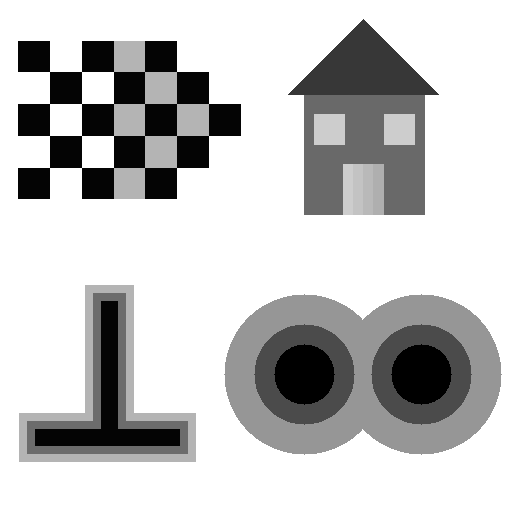
\includegraphics[width=0.5\textwidth]{../image-plots/edgetest_23.png}
    \caption{Η δεδομένη εικόνα εισόδου}
    \label{fig:edge-test}
\end{figure}

\begin{figure}[h!]
    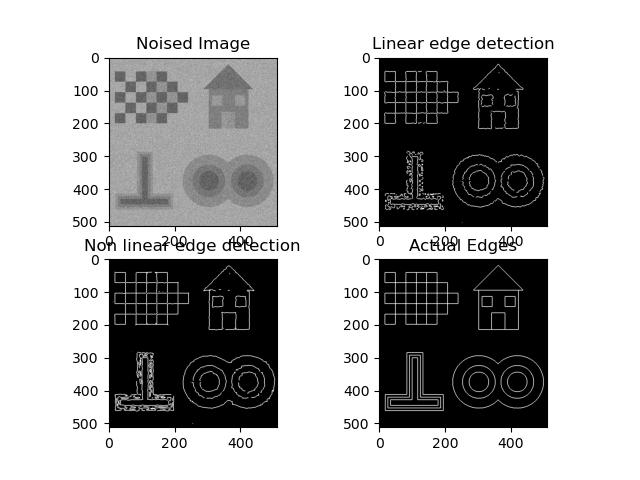
\includegraphics[width=\textwidth]{../image-plots/edges-intro0.jpg}
    \caption{Θόρυβος \eng{PSNR} 10\eng{dB}}
    \label{fig:noise 10db}
\end{figure}
\FloatBarrier

Όταν η εικόνα \ref{fig:edge-test} θορυβήθηκε με θόρυβο 10 \eng{dB PSNR}, τα αποτελέσματα ήταν αυτά που φαίνονται στην \ref{fig:noise 10db} και οι βαθμολογίες στο κριτήριο ποιότητας οι ακόλουθες:

\begin{equation}
    \begin{gathered}
        C_{10db-lin} = 0.6182010279466628\\
        C_{10db-non} = 0.7362110886293316\\
    \end{gathered}
\end{equation}

Ενώ όταν η εικόνα θορυβήθηκε με θόρυβο 20 \eng{dB PSNR}, τα αποτελέσματα ήταν:

\begin{figure}[h]
        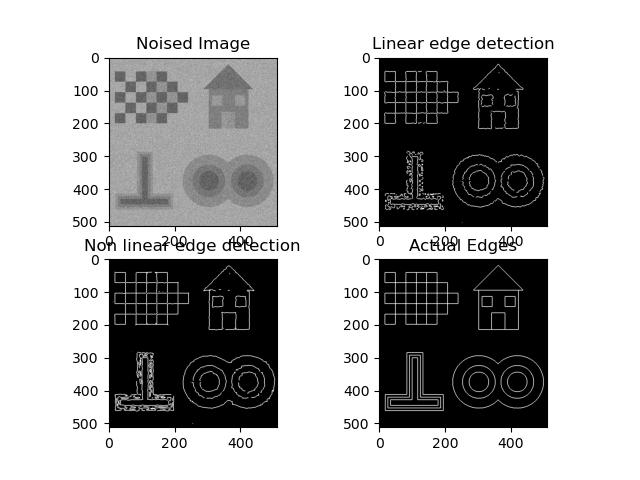
\includegraphics[width=\textwidth]{../image-plots/edges-intro0.jpg}
        \caption{Θόρυβος \eng{PSNR} 20\eng{dB}}
\end{figure}
\FloatBarrier

Με κριτήριο ποιότητας:

\begin{equation}
    \begin{gathered}
        C_{20db-lin} = 0.9375887192342924\\
        C_{20db-non} = 0.9671201094187654\\
    \end{gathered}
\end{equation}

Τα αποτελέσματα επιτεύχθηκαν με τις ακόλουθες παράμετρους:

\begin{equation}
    \begin{gathered}
        \sigma = \begin{bmatrix}3 & 1.5 \end{bmatrix},
        \theta = \begin{bmatrix}0.2 & 0.2 \end{bmatrix},
        \theta_{real} = 0,08\\
    \end{gathered}
\end{equation}

Παρατηρείται ότι η επίδραση του θορύβου είναι καθοριστική, καθώς στην εικόνα με τον λίγοτερο θόρυβο επιτυγχάνεται καλύτερη βαθμολογία στο ποιοτικό κριτήριο. Επίσης, φαίνεται ότι η μη γραμμική μέθοδος πετυχαίνει καλύτερα αποτελέσματα σε κάθε περίπτωση.

\subsection{Εφαρμογή των Αλγορίθμων Ανίχνευσης Ακμών σε Πραγματικές Εικόνες}

Η ίδια συνάρτηση χρησιμοποιήθηκε και για την ανίχνευση ακμών στην πραγματική εικόνα του \eng{Kyoto}, όπως φαίνεται στην εικόνα \ref{fig:kyoto}.

\begin{figure}[h]
    \centering
    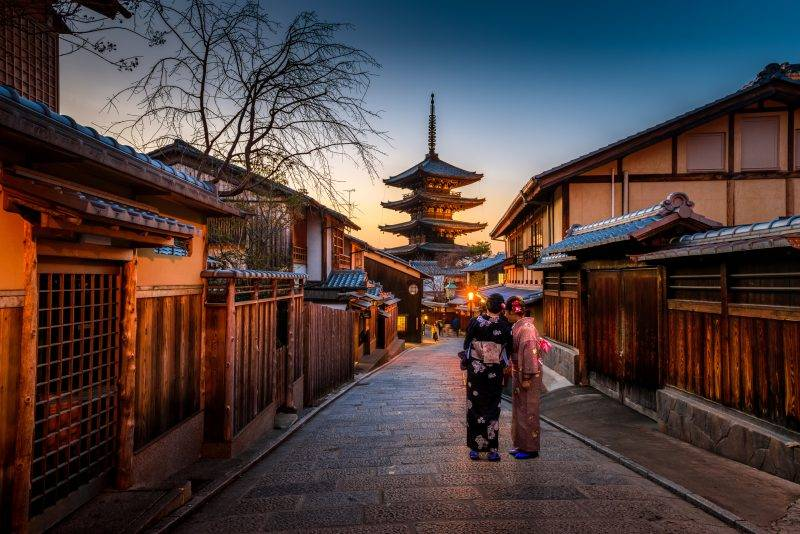
\includegraphics[width=0.5\textwidth]{../image-plots/kyoto_edges.jpg}
    \caption{Η πραγματική φωτογραφιά του \eng{Kyoto}}
    \label{fig:kyoto}
\end{figure}
\begin{figure}[h]
    \centering
    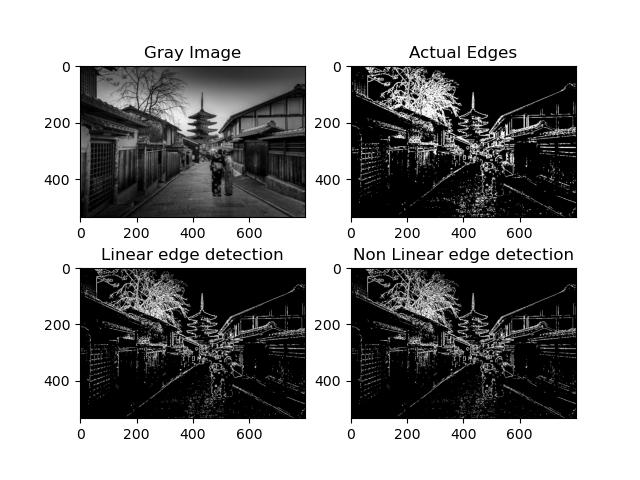
\includegraphics[width=0.9\textwidth]{../image-plots/edges-real.jpg}
    \caption{Ανίχνευση ακμών στην πραγματική φωτογραφιά του \eng{Kyoto}}
    \label{fig:kyoto-edges}
\end{figure}
\FloatBarrier

Η επεξεργασία έγινε με τις παραμέτρους:

\begin{equation}
    \begin{gathered}
        \sigma = 0.3, \theta = 0.2, \theta_{real} = 0.23 \\
    \end{gathered}
\end{equation}

και πέτυχε τις βαθμολογίες:

\begin{equation}
    \begin{gathered}
        C_{lin} = 0.818604135617401\\
        C_{non} = 0.8188562865181751
    \end{gathered}
\end{equation}

Τα δε οπτικά αποτελέσματα φαίνονται στην εικόνα \ref{fig:kyoto-edges}. Τόσο από την βαθμολογία στο ποιοτικό κριτήριο όσο και οπτικά, φαίνεται ότι αμφότερες η γραμμική και η μη γραμμική μέθοδος έδωσαν πολύ καλά αποτελέσματα.

\section{Μέρος 2ο}

Στο σημείο αυτό της εργασίας θα επιχειρηθεί η ανίχνευση διαφόρων χαρακτηριστικών, τόσο σε μία μόνο κλίμακα όσο και σε πολλαπλές κλίμακες.

\subsection{Ανίχνευση Γωνιών}

Πρώτα επιχειρείται ανίχνευση γωνιών. Θα παρουσιαστεί η μεθοδολογία και ταυτοχρόνως τα βήματα της επεξεργασίας, για να γίνει σαφής.

Αρχικά υπολογίζεται ο δομικός τανυστής \eng{\textbf{J}} και οι ιδιοτιμές του. 

\begin{equation}
    \begin{gathered}
        J_1(x, y) = G_{\rho} * \left(\frac{\partial I_\sigma}{\partial x} \cdot \frac{\partial I_\sigma}{\partial x} \right)(x, y)\\
        J_2(x, y) = G_{\rho} * \left( \frac{\partial I_\sigma}{\partial x} \cdot \frac{\partial I_\sigma}{\partial y} \right)(x, y)\\
        J_3(x, y) = G_{\rho} * \left( \frac{\partial I_\sigma}{\partial y} \cdot \frac{\partial I_\sigma}{\partial y} \right)(x, y)\\
        \lambda_{\pm}(x, y) = \frac{1}{2} \left(J_1 + J_2 \pm \sqrt{\left (J_1 - J_3\right)^2 + 4J_2^2} \right)
    \end{gathered}
\end{equation}

Οι ιδιοτιμές περιέχουν χρήσιμη πληροφορία σχετικά με τις ακμές και τις γωνίες της εικόνας. Παρακάτω, στην εικόνα \ref{fig:kyoto-eigenvalues}, δίνεται η απεικόνισή τους ως γκρίζες εικόνες.

\begin{figure}[h]
    \centering
    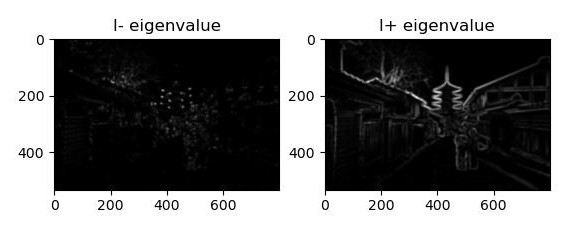
\includegraphics[width=\textwidth]{../image-plots/corner-detection-eigenvalues-scaled.jpg}
    \caption{Απεικόνιση των ιδιοτιμών της εικόνας ως γκρίζες εικόνες}
    \label{fig:kyoto-eigenvalues}
\end{figure}
\FloatBarrier

Φαίνεται ότι η εικόνα η αντιστοιχούσα στην ιδιοτιμή ''-`` αποτυπώνει έντονα τις απολήξεις του πύργου, δηλαδή τις αιχμηρές γωνίες, ενώ η εικόνα αντιστοιχούσα στην ιδιοτιμή ``+'' αποτυπώνει έντονα τα περιγράμματα, δηλαδή τις ακμές.

Στην συνέχεια, εξάγεται ένα κριτήριο γωνιότητας συναρτήσει των ιδιοτιμών και μίας σταθεράς $k$:

\begin{equation}
    R(x, y) = \lambda_{-}\lambda_{+} - k\cdot\left(\lambda_{-} + \lambda_{+}\right)^2
\end{equation}

Τέλος, επιλέγονται ως γωνίες τα σημεία αυτά τα οποία μεγιστοποιούν το κριτήριο εντός τετραγωνικών παραθύρων και αποδίδουν στο κριτήριο γωνιότητας τιμή μεγαλύτερη από ένα κατώφλι.

\begin{equation}
    \begin{gathered}
        R(x, y) > \theta_{corn} \cdot R_{max} 
    \end{gathered}
\end{equation}

Το αποτέλεσμα εφαρμογής αυτών των συνθηκών στην εικόνα-κριτήριο $R$, για τις παραμέτρους $\sigma = 2, \rho = 2.5, k = 0.05, \theta_{corn} = 0.1$ είναι το ακόλουθο:
       

\begin{figure}[h]
    \centering
    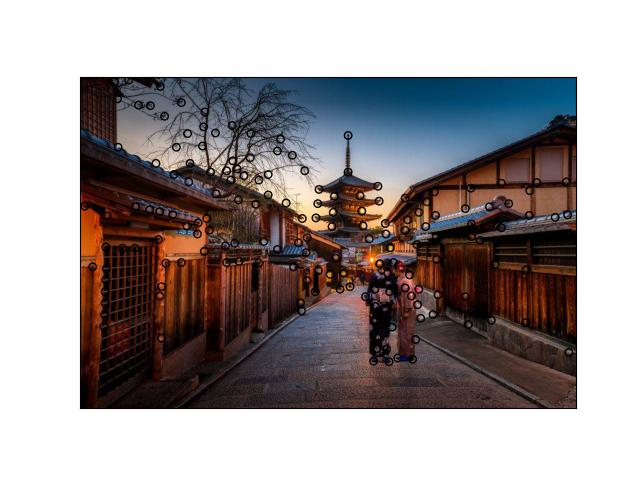
\includegraphics[width=\textwidth]{../image-plots/corner-detection.jpg}
    \caption{Ανίχνευση γωνιών στην εικόνα \eng{Kyoto}}
    \label{fig:kyoto-corners}
\end{figure}
\FloatBarrier

Φαίνεται ότι έχουν εντοπιστεί με επιτυχία πολλές γωνίες, ειδικά οι αιχμηρές απολίξεις του πύργου αλλά και οι ορθές γωνίες οι σχηματιζόμενες από τους πασάλους των κτιρίτων. Ωστόσο, έχουν αναγνωριστει ως γωνίες και ανεπιθύμητα σημεία, όπως τα κλαδιά του δέντρου. Επομένως, συμπεραίνεται ότι η μέθοδος είναι αποτελεσματική αλλά έχει περιθώριο βελτίωσης.

\subsection{Πολυκλιμακωτή Ανίχνευση Γωνιών}

Ένα σημαντικό μειονέκτημα της προηγούμενης μεθόδου ήταν ότι περιοριζόταν σε μία μόνο κλίμακα, αφού δεχόταν μόνο ένα ζευγάρι παραμέτρων $(\sigma, \rho)$. Η ιδέα είναι να εφαρμοσθεί η ίδια μέθοδος Ν φορές, κλιμακώνοντας γεωμετρικά κάθε φορά τις παραμέτρους με μία παραμέτρο κλίμακας $s$. Δηλαδή, η επεξεργασία θα γίνεται με τις παραμέτρους:

 \begin{equation}
    \begin{gathered}
        \sigma_0, \sigma_1, ..., \sigma_{N-1} = s^{0}\sigma_0, s^{1}\sigma_0, ..., \sigma^{N-1}\sigma_0 \\
        \rho_0, \rho_1, ..., \rho_{N-1} = s^{0}\rho_0, s^{1}\rho_0, ..., \rho^{N-1}\rho_0 
    \end{gathered}
\end{equation}

Λόγω των πολλαπλών κλιμάκων, θα επιλεχθούν πολλά σημεία τα οποία έχουν την ίδια πιθανότητα σφάλματος όπως προηγουμένως. Για αυτόν τον λόγο, επιλέγονται τελικά αυτά τα σημεία-γωνίες τα οποία μεγιστοποιούν κάποιο κριτήριο σε μία περιοχή κλιμάκων. Εν προκειμένω, το κριτήριο επιλέγεται να είναι η κανονικοποιημένη Λαπλασιανή της Γκαουσιανής.

\begin{equation}
    \left| LoG(x, y, \sigma_i) \right| = \sigma_i^2 \left|L_xx(x,y, \sigma_i) + L_yy(x, y, \sigma_i) \right|
\end{equation}

Ουσιαστικά, το σκεπτικό είναι ότι μία γωνία οφείλει να εντοπίζεται τουλάχιστον σε μία μικρή περιοχή κλιμάκων, όχι μόνο σε μία διακεκριμένη κλίμακα. Το αποτέλεσμα της πολυκλιμακωτής μεθόδου στην ίδια εικόνα φαίνεται παρακάτω:

\begin{figure}[h]
    \centering
    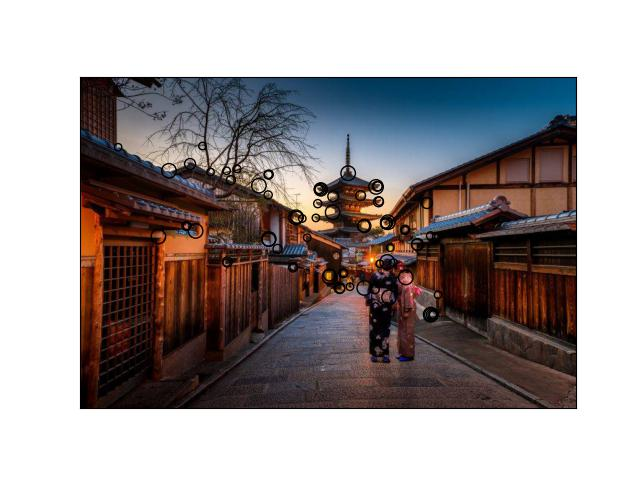
\includegraphics[width=\textwidth]{../image-plots/corner-detection-multiscale.jpg}
    \caption{Πολυκλιμακωτή ανίχνευση γωνιών στην εικόνα \eng{Kyoto}}
    \label{fig:kyoto-corners-multiscale}
\end{figure}
\FloatBarrier

Παρατηρείται, ότι εντοπίζονται λιγότερες γωνίες απ'ό,τι προηγουμένως. Επιθεωρώντας την εικόνα, παρατηρείται ότι έπαψαν να εντοπίζονται κάποιες ψεύτικες γωνίες, κυρίως αυτές στα ψιλά κλαδιά του δέντρου, παρασέρνοντας όμως και λίγες πραγματικές, όπως αυτές στον πύργο. Ωστόσο, εξακολουθούν να εντοπίζονται εν πολλοίς οι πραγματικές γωνίες, και μάλιστα με μεγαλύτερη βεβαιότητα, αφού περικλείονται από κύκλους διαφόρων κλιμάκων. Συμπερασματικά, η μέθοδος αυτή είναι σαφώς βελτίωση της προηγούμενης, με αντίτιμο μεγαλύτερη υπολογιστική πολυπλοκότητα.

\subsection{Ανίχνευση \eng{Blobs}}

Η ανίχνευση \eng{blobs} αναφέρεται γενικώς στην ανίχνευση περιοχών με κάποια ομοιογένεια. Οι περιοχές αυτές βρίσκονται χρήσει των μερικών παραγώγων δευτέρας τάξεως της εξομαλυμένης εικόνας. Συγκεκριμένα,  δεδομένου του Χεσιανού πίνακα:

\begin{equation}
    H(x, y) = \begin{bmatrix} L_{xx}(x, y, \sigma) & L_{xy}(x, y, \sigma) \\
                L_{xy}(x, y, \sigma) & L_{yy}(x, y, \sigma)\end{bmatrix}
\end{equation}

Το κριτήριο για τον εντοπισμό περιοχών ομοιογένειας είναι απλώς ο μηδενισμός της ορίζουσας:

\begin{equation}
    \begin{gathered}
        R(x, y) = \det\left| H(x, y) \right|\\
        (x, y) = \underset{x, y} {\arg} \left( R(x, y) = 0 \right)
    \end{gathered}
\end{equation}

Επομένως, αναπτύσσεται μεθοδολογία πλήρως ανάλογη με την μεθοδολογία για την ανίχνευση ακμών. Δηλαδή, εξομαλύνεται η εικόνα, υπολογίζεται ο Χεσιανός πίνακας και το κριτήριο $R(x, y)$, εντοπίζονται τα σημεία μηδενισμού και επιλέγονται αυτά τα οποία έχουν τιμή στην εικόνα μεγαλύτερη από κάποιο κατώφλι.

Η μέδοδος εφαρμόζεται στην εικόνα \eng{Up}, από την ομώνυμη ταινία της \eng{Pixar}, και σε μία εικόνα ανθρωπίνων κυττάρων. Πρώτη θα εξεταστεί η εφαρμογή στην εικόνα \eng{Up}.


\begin{figure}[h]
    \begin{subfigure}{.5\textwidth}
        \centering
        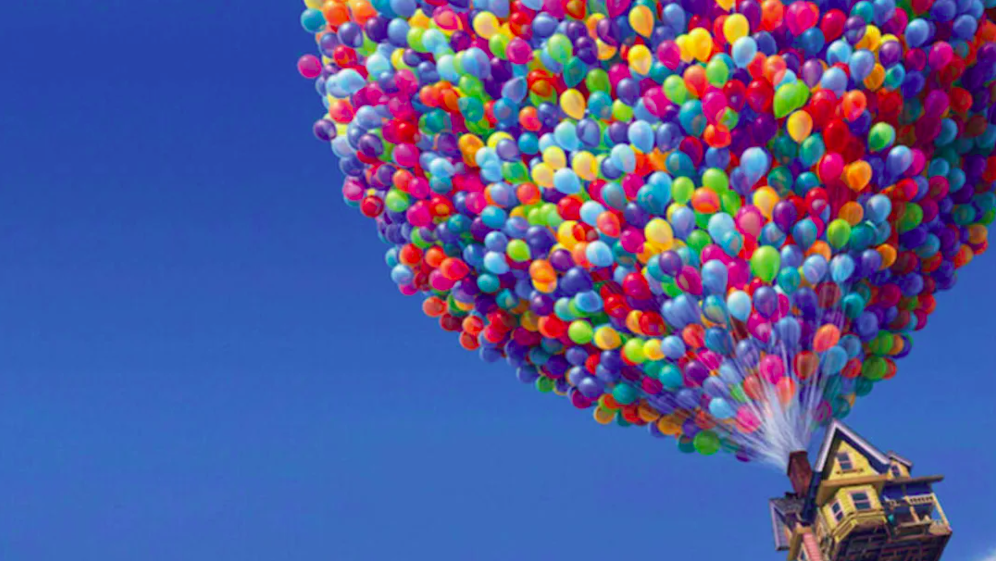
\includegraphics[width=\textwidth]{../image-plots/up.png}
        \caption{Η εικόνα \eng{Up}}
        \label{fig:up}
    \end{subfigure}
    \begin{subfigure}{.5\textwidth}
        \centering
        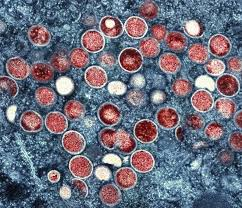
\includegraphics[width=0.8\textwidth]{../image-plots/cells.jpg}
        \caption{Η εικόνα ανθρωπίνων κυττάρων}
        \label{fig:up}
    \end{subfigure}
    \caption{Οι αρχικές εικόνες για την ανίχνευση \eng{blobs}}
\end{figure}
\FloatBarrier

Παρακάτω, στην εικόνα \ref{fig:up-blobs} φαίνονται τα αποτελέσματα για παραμέτρους $\sigma = 2.5, \theta = 0.005$

\begin{figure}[h]
    \centering
    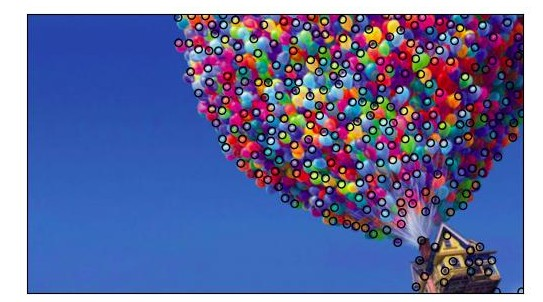
\includegraphics[width=\textwidth]{../image-plots/blob-detection-up-scaled.jpg}
    \caption{Aνίχνευση \eng{blobs} στην εικόνα \eng{Up}}
    \label{fig:up-blobs}
\end{figure}
\FloatBarrier

Παρατηρείται, ότι αν και το κατώφλι για την αποδοχή της περιοχής ομοιογένειας είναι πολύ χαμηλό, τα αποτελέσματα είναι πολύ ικανοποιητικά. Συγκεκριμένα, εντοπίζονται οι περιοχές στα μπαλόνια οι οποίες αντανακλούν το φως του ηλίου και έχουν χαρακτηριστική λευκή λάμψη. Επιπλέον, εντοπίζονται οι περιοχές μεταξύ των μπαλονιών στις οποίες υπάρχει σκοτάδι

Εξετάζεται τώρα η εφαρμογή της μεθόδου στην εικόνα των κυττάρων.

Τα αποτελέσματα για τις ίδιες παραμέτρους με πριν είναι αυτά που φαίνονται στην εικόνα \ref{fig:cells-bad}

\begin{figure}[h]
    \centering
    \begin{subfigure}{.49\textwidth}
        \centering
        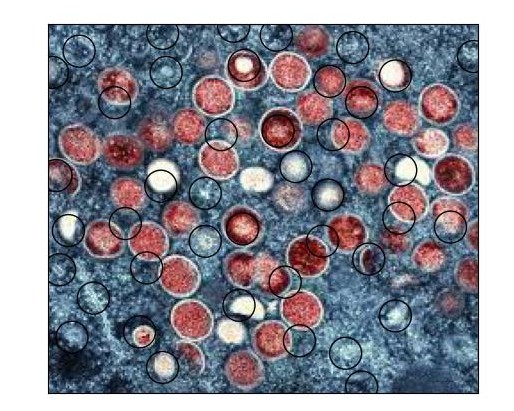
\includegraphics[width=\textwidth]{../image-plots/blob-detection-cells-bad-scaled.jpg}
        \caption{Aνίχνευση \eng{blobs} στην εικόνα ανθρωπίνων κυττάρων χαμηλό κατώφλι}
        \label{fig:cells-bad}
    \end{subfigure}
    \begin{subfigure}{.49\textwidth}
        \centering
        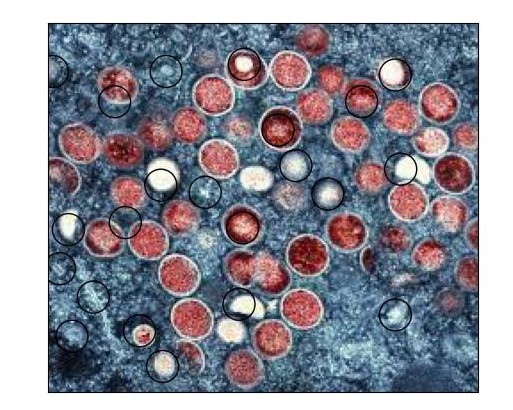
\includegraphics[width=\textwidth]{../image-plots/blob-detection-cells-good-scaled.jpg}
        \caption{Aνίχνευση \eng{blobs} στην εικόνα ανθρωπίνων κυττάρων υψηλό κατώφλι}
        \label{fig:cells-good}
    \end{subfigure}
\end{figure}
\FloatBarrier

Παρατηρείται, ότι αν και ανιχνεύονται επιτυχώς μερικές από τις λευκές περιοχές ομοιογένειας, ανιχνεύονται επίσης ανεπιθυμητές περιοχές. Αυτό συμβαίνει, γιατί το περιβάλλον της εικόνας είναι τραχύ, με αποτέλεσμα οποιαδήποτε ομοιογένεια να ξεχωρίζει. Αντιθέτως, ο ουρανός προηγουμένως είναι πολύ ομαλός και ομοιογενής, επομένως δεν ξεχωρίζει. Για αυτόν τον λόγο, προσαρμόζεται η παράμετρος $\theta \leftarrow 0.25$. Τα νέα αποτελέσματα φαίνονται στην εικόνα \ref{fig:cells-good}, όπου πλέον ανιχνεύονται σαφώς λίγοτερες περιοχές ομοιογένειες, αλλά ορθότερες.

\begin{figure}[h]
    \centering
    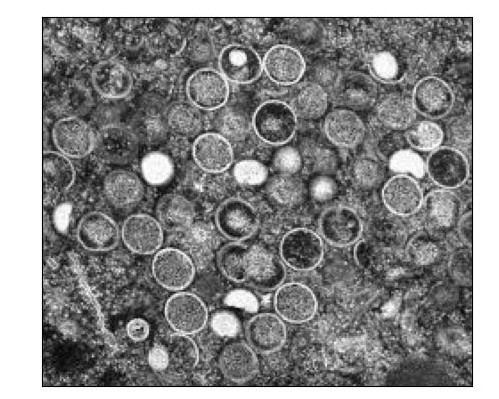
\includegraphics[width=0.8\textwidth]{../image-plots/cells-gray-scaled.jpg}
    \caption{Η εικόνα των κυττάρων γκρίζα}
    \label{fig:cells-gray}
\end{figure}
\FloatBarrier

Αξιοσημειώτο είναι το γεγονός ότι οι ερυθρές περιοχές γενικώς δεν ανιχνεύονται, σίγουρα όχι στον ίδιο βαθμό με τις λευκές. Αυτό συμβαίνει γιατί η επεξεργασία γίνεται στην γκρίζα μορφή της εικόνας, επομένως η χρωματική διαφορά απαλείφεται, όπως φαίνεται στην εικόνα \ref{fig:cells-gray}. Εφόσον η υφή είναι η ίδια, ανεξαρτήτως χρώματος, γίνεται σαφές ότι δεν μπορούν να διακριθούν στον ίδιο βαθμό με τις λευκές. Εκτός από αυτό, συμπεραίνεται ότι σε τραχύ περιβάλλον πρέπει να αυξηθεί το κατώφλι αποδοχής σημείων.

\subsection{Πολυκλιμακωτή Ανίχνευση \eng{Blobs}}

Για την βελτίωση της μεθόδου χρησιμοποιούνται τώρα πολλαπλές κλίμακες, σε πλήρη αναλογία με την πολυκλιμακωτή ανίχνευση γωνιών.

Στην εικόνα \ref{fig:up-multiscale} φαίνονται τα αποτελέσματα στην εικόνα \eng{Up} για τις τιμές παραμέτρων $\sigma = 3, \theta = 0.05, s = 1.1, N = 8$. Παρατηρείται ότι εντοπίζονται \eng{blobs} ποικίλλων μεγεθών, στα οποία περιλαμβάνονται τόσο ολόκληρα μπαλόνια όσο και απλές αντανακλάσεις φωτός, όπως προηγουμένως.
\begin{figure}[h]
    \centering
    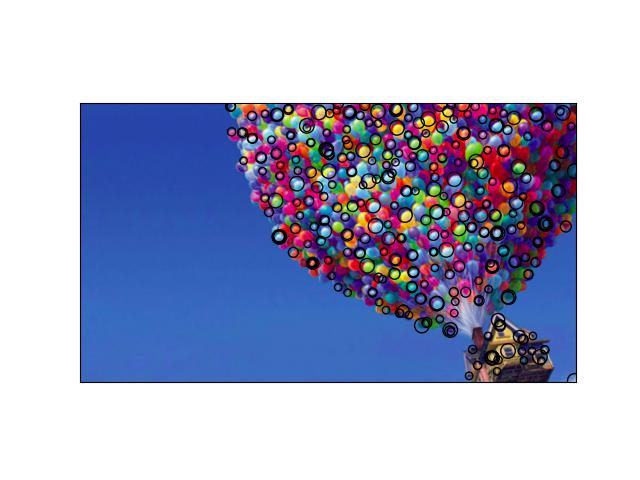
\includegraphics[width=\textwidth]{../image-plots/blob-detection-multiscale-up.jpg}
    \caption{Πολυκλιμακωτή ανίχνευση \eng{blobs} στην εικόνα \eng{Up}}
    \label{fig:up-multiscale}
\end{figure}
\FloatBarrier

Στην εικόνα \ref{fig:cells-multiscale-bad} φαίνεται το αποτέλεσμα της πολυκλιμακωτής ανίχνευσης \eng{blobs} για τις τιμές παραμέτρων $\sigma = 3, \theta = 0.05, s = 1.1, N = 8$. Η ανίχνευση γίνεται σε 8 κλίμακες του $\sigma = 3$ με παράγοντα το 1.1 και χαμηλό κατώφλι.Αντιστοίχως, στην εικόνα \ref{fig:cells-multiscale-good} φαίνεται το αποτέλεσμα της πολυκλιμακωτής ανίχνευσης \eng{blobs} για τις τιμές παραμέτρων $\sigma = 3, \theta = 0.15, s = 1.1, N = 8$. Δηλαδή, η ανίχνευση γίνεται σε 8 κλίμακες  του $\sigma = 3$ και με υψηλότερο κατώφλι, με παράγοντα το 1.1.

Στην δε εικόνα \ref{fig:cells-multiscale-pair} παρατηρείται, ότι μειώνοντας το κατώφλι, όπως και στην μονοκλιμακωτή ανίχνευση, απορρίπτονται επιτυχώς κάποια ανεπιθύμητα \eng{blobs}. Μάλιστα, αυτό γίνεται εν προκειμένω με μεγαλύτερη επιτυχία, καθώς εξακολουθούν να ανιχνεύονται όλες οι λευκές περιοχές. Δεν απορρίπτεται, δηλαδή, κατά λάθος, κάποιο επιθυμητό \eng{blob}. Επομένως, συμπεραίνεται ότι η επέκταση της μεθόδου σε πολλαπλές κλίμακες είναι ευεργετική.

\begin{figure}[h]
    \centering
    \begin{subfigure}{\textwidth}
    \centering
    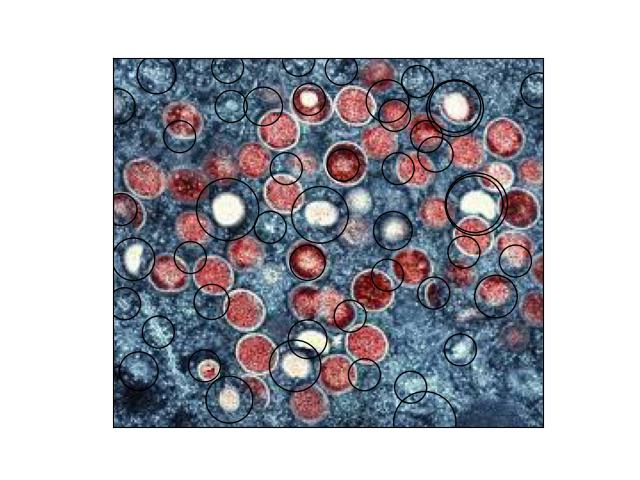
\includegraphics[width=\textwidth]{../image-plots/blob-detection-multiscale-cells-bad.jpg}
    \caption{Χαμηλό κατώφλι}
    \label{fig:cells-multiscale-bad}
    \end{subfigure}
    \begin{subfigure}{\textwidth}
    \centering
    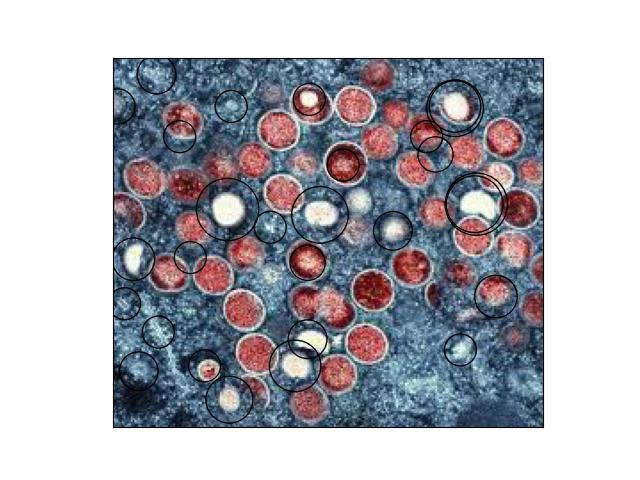
\includegraphics[width=\textwidth]{../image-plots/blob-detection-multiscale-cells-good.jpg}
    \caption{Υψηλό κατώφλι}
    \label{fig:cells-multiscale-good}
    \end{subfigure}
    \caption{Πολυκλιμακωτή ανίχνευση \eng{blobs} σε κύτταρα}
    \label{fig:cells-multiscale-pair}
\end{figure}
\FloatBarrier

\subsection{Επιτάχυνση Ανίχνευσης \eng{Blobs}}

Η παραπάνω μέθοδος μπορεί να επιταχυνθεί \footnote{Σημειώνεται ότι η παρατηρούμενη επιτάχυνση εξαρτάται από την υλοποίηση της απλής μεθόδου ανίχνευσης \eng{blobs}. Βλέπε \ref{section:details}.} χρήσει ολοκληρωτικών εικόνων και \eng{box filter}. Συγκεκριμένα, ο υπολογισμός των μερικών παραγώγων μέχρι στιγμής απαιτούσε την συνέλιξη φίλτρων με την εκάστοτε εικόνα, γεγονός που τον καθιστούσε υπολογιστικά ακριβό.

Οι ολοκληρωτικές εικόνες είναι μία τεχνική η οποία επιτρέπει των υπολογισμό συνελίξεων με την εικόνα σε χρόνο ανεξάρτητο του πυρήνα και εξαρτώμενο μόνο από το μέγεθος της εικόνας. Αυτό συμβαίνει, γιατί, χρήσει ολοκληρωτικών εικόνων, το άθροισμα των \eng{pixels} μίας ορθογώνιας περιοχής μπορεί να υπολογιστεί σε σταθερό χρόνο. Για να επιτευχθεί, όμως, η επιτάχυνση αυτή, χρησιμοποιείται μία προσέγγιση της παραγώγου. Επομένως, πρόκειται για προσεγγιστική μέθοδο και αναμένονται αποκλίσεις από τα προηγούμενα αποτελέσματα.

Στην εικόνα \ref{fig:ii} φαίνονται τα αποτελέσματα της απόπειρας επιτάχυνσης της ανίχνευσης \eng{blobs} στις ίδιες εικόνες όπως προηγουμένως, στην οποία χρησιμοποιήθηκαν οι ίδιες ακριβώς παράμετροι όπως και στην απλή μέθοδο.

Στην εικόνα \ref{fig:up-ii}, όπου χρησιμοποιείται μικρή τιμή της παραμέτρου $\sigma$, τα αποτελέσματα είναι πολύ ικανοποιητικά, καθώς εντοπίζονται επιτυχώς οι αντανακλάσεις φωτός επάνω στα μπαλόνια και, φυσικά, δεν αντιμετωπίζονται εσφαλμένες περιοχές ομοιογένειας.

Στην δε εικόνα \ref{fig:cells-ii}, όπου χρησιμοποιείται μεγαλύτερη τιμή της παραμέτρου  $\sigma$, τα αποτελέσματα δεν είναι το ίδιο ικανοποιητικά. Συγκεκριμένα, παρατηρείται ότι ανιχνεύονται μερικά ανεπιθύμητα \eng{blobs}, ωστόσο ανιχνεύονται και μερικά ορθώς. Επομένως, είναι εμφανές το γεγονός ότι η επιτάχυνση οφείλεται σε προσέγγιση.

\begin{figure}[h]
    \centering
    \begin{subfigure}{\textwidth}
        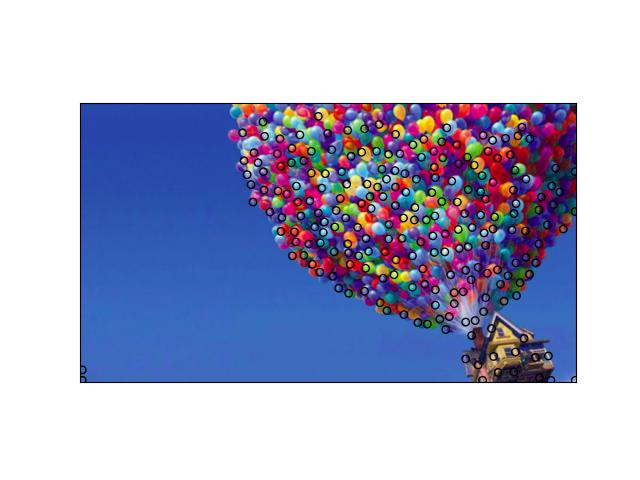
\includegraphics[width=\textwidth]{../image-plots/blob-detection-ii-up.jpg}
        \caption{Αποτέλεσμα στην εικόνα \eng{Up}}
        \label{fig:up-ii}
    \end{subfigure}
    \begin{subfigure}{\textwidth}
        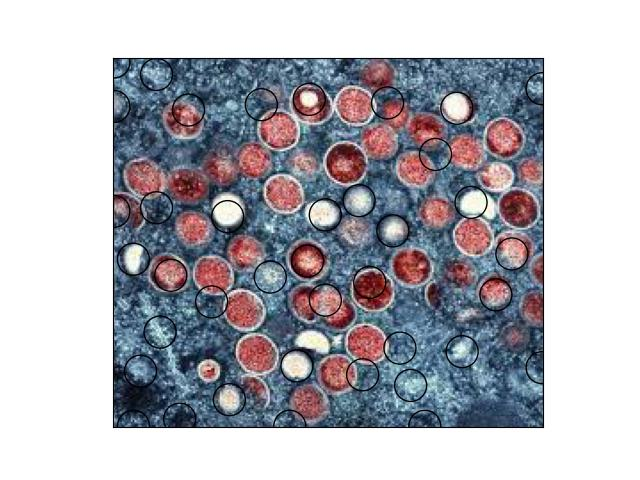
\includegraphics[width=\textwidth]{../image-plots/blob-detection-ii-cells.jpg}
        \caption{Αποτέλεσμα στην εικόνα κυττάρων}
        \label{fig:cells-ii}
    \end{subfigure}
    \caption{Προσέγγιση ανίχνευσης \eng{blobs} με ολοκληρωτικές εικόνες}
    \label{fig:ii}
\end{figure}
\FloatBarrier

\subsection{Επιτάχυνση Πολυκλιμακωτής Ανίχνευση \eng{Blobs}}

Τα ίδια συμπεράσματα προκύπτουν και για την πολυκλιμακωτή ανίχνευση.

\begin{figure}[h]
    \centering
    \begin{subfigure}{0.7\textwidth}
        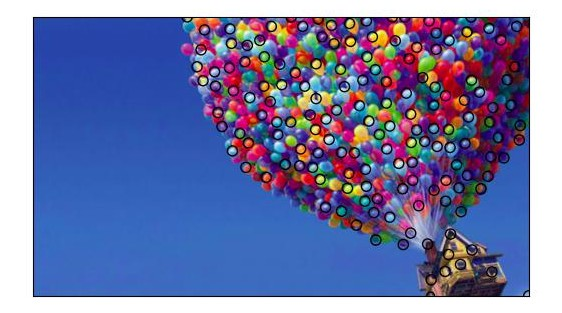
\includegraphics[width=\textwidth]{../image-plots/blob-detection-multiscale-ii-up-scaled.jpg}
        \caption{Αποτέλεσμα στην εικόνα \eng{Up}}
        \label{fig:cells-multiscale-ii}
    \end{subfigure}
    \begin{subfigure}{0.7\textwidth}
        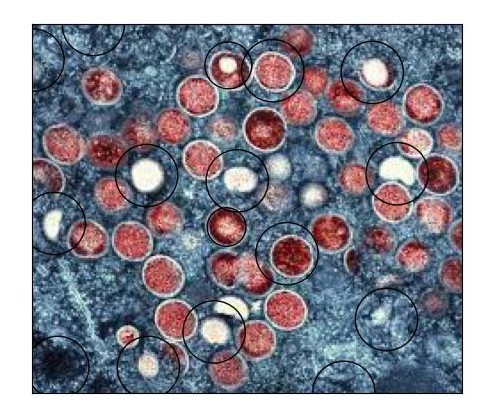
\includegraphics[width=\textwidth]{../image-plots/blob-detection-multiscale-ii-cells-scaled.jpg}
        \caption{Αποτέλεσμα στην εικόνα κυττάρων}
        \label{fig:cells-multiscale-ii}
    \end{subfigure}
    \caption{Προσέγγιση πολυκλιμακωτής ανίχνευσης \eng{blobs} με ολοκληρωτικές εικόνες}
\end{figure}
\FloatBarrier


\newpage
\section{Παράρτημα}
\subsection{Επιτάχυνση χρήσει ολοκληρωτικών εικόνων και \eng{box filters}}
\label{section:details}

Η παρατηρούμενη επιτάχυνση εξαρτάται και από την υλοποίηση τηςαπλής μεθόδου ανίχνευσης \eng{blobs}. Συγκεκριμένα, αν ο υπολογισμός των μερικών παραγώγων είχε γίνει χρήσει ''χειροποίητης`` συνάρτησης συνελίξεως δύο διαστάσεων, τότε η επιτάχυνση γίνεται αμέσως εμφανής. Ωστόσο, αν ο υπολογισμός μερικών παραγώγων είχε γίνει χρήσει έτοιμης συνάρτησης συνέλιξης από την βιβλιοθήκη \eng{cv2}, τότε η επιτάχυνση δεν θα είναι εμφανής. Αυτό συμβαίνει γιατί, κατόπιν μετρήσεων για διάφορες τιμές τις παραμέτρου $\sigma$, παρατηρήθηκε ότι η ταχύτητα της συνάρτησης  \eng{cv2.filter2D} ήταν πρακτικά σταθερή. Το ίδιο παρατηρήθηκε και για την υλοποίηση χρήσει ολοκληρωτικών εικόνων και \eng{box filters}. Η δε ''χειροκίνητη`` υλοποίηση της διδιάστασης συνέλιξης εμφάνισε τετραγωνική χρονική εξάρτηση από την παράμετρο $\sigma$, όπως αναμενόταν. Τα συμπεράσματα παρουσιάζονται συνοπτικά στο ακόλουθο γράφημα \ref{fig:grad-comparison}. Αξιοσημειώτο είναι ότι, για την δίκαιη σύγκριση των αποτελεσμάτων, χρησιμοποιήθηκε ο \eng{Just-in-Time} μεταγλωττιστής \eng{Numba} για την βελτιστοποίηση των βρόχων \eng{for} στην υλοποίηση της διδιάστατης συνέλιξης. Παρ'όλα αυτά, η διαφορά στην απόδοση παραμένει σημαντική.

\begin{figure}[h]
    \centering
    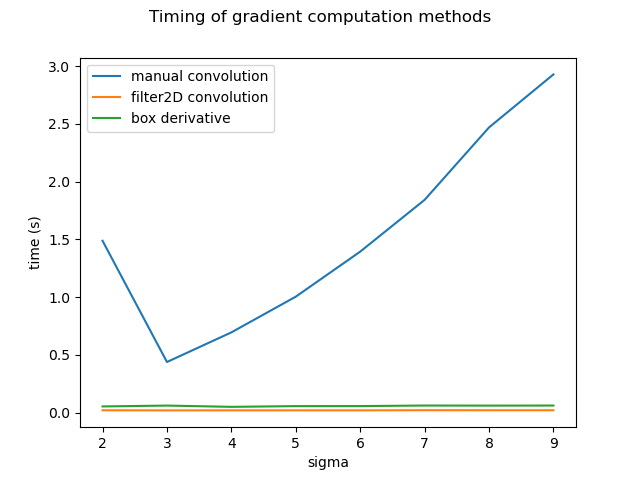
\includegraphics[width=\textwidth]{../image-plots/grad-comparison.png}
    \caption{Σύγκριση ταχύτητας διαφόρων υλοποιήσεων υπολογισμού μερικών παραγώγων}
    \label{fig:grad-comparison}
\end{figure}
\FloatBarrier


\end{document}

